% Options for packages loaded elsewhere
\PassOptionsToPackage{unicode}{hyperref}
\PassOptionsToPackage{hyphens}{url}
%
\documentclass[
]{article}
\usepackage{amsmath,amssymb}
\usepackage{lmodern}
\usepackage{iftex}
\ifPDFTeX
  \usepackage[T1]{fontenc}
  \usepackage[utf8]{inputenc}
  \usepackage{textcomp} % provide euro and other symbols
\else % if luatex or xetex
  \usepackage{unicode-math}
  \defaultfontfeatures{Scale=MatchLowercase}
  \defaultfontfeatures[\rmfamily]{Ligatures=TeX,Scale=1}
\fi
% Use upquote if available, for straight quotes in verbatim environments
\IfFileExists{upquote.sty}{\usepackage{upquote}}{}
\IfFileExists{microtype.sty}{% use microtype if available
  \usepackage[]{microtype}
  \UseMicrotypeSet[protrusion]{basicmath} % disable protrusion for tt fonts
}{}
\makeatletter
\@ifundefined{KOMAClassName}{% if non-KOMA class
  \IfFileExists{parskip.sty}{%
    \usepackage{parskip}
  }{% else
    \setlength{\parindent}{0pt}
    \setlength{\parskip}{6pt plus 2pt minus 1pt}}
}{% if KOMA class
  \KOMAoptions{parskip=half}}
\makeatother
\usepackage{xcolor}
\usepackage[margin=1in]{geometry}
\usepackage{color}
\usepackage{fancyvrb}
\newcommand{\VerbBar}{|}
\newcommand{\VERB}{\Verb[commandchars=\\\{\}]}
\DefineVerbatimEnvironment{Highlighting}{Verbatim}{commandchars=\\\{\}}
% Add ',fontsize=\small' for more characters per line
\usepackage{framed}
\definecolor{shadecolor}{RGB}{248,248,248}
\newenvironment{Shaded}{\begin{snugshade}}{\end{snugshade}}
\newcommand{\AlertTok}[1]{\textcolor[rgb]{0.94,0.16,0.16}{#1}}
\newcommand{\AnnotationTok}[1]{\textcolor[rgb]{0.56,0.35,0.01}{\textbf{\textit{#1}}}}
\newcommand{\AttributeTok}[1]{\textcolor[rgb]{0.77,0.63,0.00}{#1}}
\newcommand{\BaseNTok}[1]{\textcolor[rgb]{0.00,0.00,0.81}{#1}}
\newcommand{\BuiltInTok}[1]{#1}
\newcommand{\CharTok}[1]{\textcolor[rgb]{0.31,0.60,0.02}{#1}}
\newcommand{\CommentTok}[1]{\textcolor[rgb]{0.56,0.35,0.01}{\textit{#1}}}
\newcommand{\CommentVarTok}[1]{\textcolor[rgb]{0.56,0.35,0.01}{\textbf{\textit{#1}}}}
\newcommand{\ConstantTok}[1]{\textcolor[rgb]{0.00,0.00,0.00}{#1}}
\newcommand{\ControlFlowTok}[1]{\textcolor[rgb]{0.13,0.29,0.53}{\textbf{#1}}}
\newcommand{\DataTypeTok}[1]{\textcolor[rgb]{0.13,0.29,0.53}{#1}}
\newcommand{\DecValTok}[1]{\textcolor[rgb]{0.00,0.00,0.81}{#1}}
\newcommand{\DocumentationTok}[1]{\textcolor[rgb]{0.56,0.35,0.01}{\textbf{\textit{#1}}}}
\newcommand{\ErrorTok}[1]{\textcolor[rgb]{0.64,0.00,0.00}{\textbf{#1}}}
\newcommand{\ExtensionTok}[1]{#1}
\newcommand{\FloatTok}[1]{\textcolor[rgb]{0.00,0.00,0.81}{#1}}
\newcommand{\FunctionTok}[1]{\textcolor[rgb]{0.00,0.00,0.00}{#1}}
\newcommand{\ImportTok}[1]{#1}
\newcommand{\InformationTok}[1]{\textcolor[rgb]{0.56,0.35,0.01}{\textbf{\textit{#1}}}}
\newcommand{\KeywordTok}[1]{\textcolor[rgb]{0.13,0.29,0.53}{\textbf{#1}}}
\newcommand{\NormalTok}[1]{#1}
\newcommand{\OperatorTok}[1]{\textcolor[rgb]{0.81,0.36,0.00}{\textbf{#1}}}
\newcommand{\OtherTok}[1]{\textcolor[rgb]{0.56,0.35,0.01}{#1}}
\newcommand{\PreprocessorTok}[1]{\textcolor[rgb]{0.56,0.35,0.01}{\textit{#1}}}
\newcommand{\RegionMarkerTok}[1]{#1}
\newcommand{\SpecialCharTok}[1]{\textcolor[rgb]{0.00,0.00,0.00}{#1}}
\newcommand{\SpecialStringTok}[1]{\textcolor[rgb]{0.31,0.60,0.02}{#1}}
\newcommand{\StringTok}[1]{\textcolor[rgb]{0.31,0.60,0.02}{#1}}
\newcommand{\VariableTok}[1]{\textcolor[rgb]{0.00,0.00,0.00}{#1}}
\newcommand{\VerbatimStringTok}[1]{\textcolor[rgb]{0.31,0.60,0.02}{#1}}
\newcommand{\WarningTok}[1]{\textcolor[rgb]{0.56,0.35,0.01}{\textbf{\textit{#1}}}}
\usepackage{graphicx}
\makeatletter
\def\maxwidth{\ifdim\Gin@nat@width>\linewidth\linewidth\else\Gin@nat@width\fi}
\def\maxheight{\ifdim\Gin@nat@height>\textheight\textheight\else\Gin@nat@height\fi}
\makeatother
% Scale images if necessary, so that they will not overflow the page
% margins by default, and it is still possible to overwrite the defaults
% using explicit options in \includegraphics[width, height, ...]{}
\setkeys{Gin}{width=\maxwidth,height=\maxheight,keepaspectratio}
% Set default figure placement to htbp
\makeatletter
\def\fps@figure{htbp}
\makeatother
\setlength{\emergencystretch}{3em} % prevent overfull lines
\providecommand{\tightlist}{%
  \setlength{\itemsep}{0pt}\setlength{\parskip}{0pt}}
\setcounter{secnumdepth}{-\maxdimen} % remove section numbering
\ifLuaTeX
  \usepackage{selnolig}  % disable illegal ligatures
\fi
\IfFileExists{bookmark.sty}{\usepackage{bookmark}}{\usepackage{hyperref}}
\IfFileExists{xurl.sty}{\usepackage{xurl}}{} % add URL line breaks if available
\urlstyle{same} % disable monospaced font for URLs
\hypersetup{
  pdftitle={Chapter 22: Model basic},
  pdfauthor={Dat},
  hidelinks,
  pdfcreator={LaTeX via pandoc}}

\title{Chapter 22: Model basic}
\author{Dat}
\date{2023-02-23}

\begin{document}
\maketitle

\hypertarget{model-basics}{%
\section{23. Model basics}\label{model-basics}}

\hypertarget{introduction}{%
\subsection{23.1 Introduction}\label{introduction}}

Trong model sẽ bao gồm 2 phần cần chú ý:

\begin{enumerate}
\def\labelenumi{\arabic{enumi}.}
\tightlist
\item
  Family: là dạng của model muốn sử dụng, tuyến tính hay hàm số bậc hai.
\item
  Fitted model: để fit dạng family model muốn sử dụng gần đúng nhất với
  data
\end{enumerate}

Quan trọng nhất là model ``tốt nhất'' (theo tuỳ chuẩn) không có nghĩa là
model đúng với thực tế ``true''

\begin{quote}
All models are wrong, but some are useful. - George Box
\end{quote}

\begin{quote}
For such a model there is no need to ask the question ``Is the model
true?''. If ``truth'' is to be the ``whole truth'' the answer must be
``No''. The only question of interest is ``Is the model illuminating and
useful?''.
\end{quote}

Đầu tiên load các libary cần thiết

\begin{Shaded}
\begin{Highlighting}[]
\FunctionTok{library}\NormalTok{(tidyverse)}
\end{Highlighting}
\end{Shaded}

\begin{verbatim}
## -- Attaching packages --------------------------------------- tidyverse 1.3.2 --
## v ggplot2 3.4.0     v purrr   1.0.1
## v tibble  3.1.8     v dplyr   1.1.0
## v tidyr   1.3.0     v stringr 1.5.0
## v readr   2.1.3     v forcats 1.0.0
## -- Conflicts ------------------------------------------ tidyverse_conflicts() --
## x dplyr::filter() masks stats::filter()
## x dplyr::lag()    masks stats::lag()
\end{verbatim}

\begin{Shaded}
\begin{Highlighting}[]
\FunctionTok{library}\NormalTok{(modelr)}
\FunctionTok{options}\NormalTok{(}\AttributeTok{na.action =}\NormalTok{ na.warn)}
\end{Highlighting}
\end{Shaded}

\hypertarget{model-cux1a1-bux1ea3n}{%
\subsection{23.2 Model cơ bản}\label{model-cux1a1-bux1ea3n}}

Đầu tiên xem data set của sim1 trong modelr, gồm 2 biến x và y ở dạng
continuous

\begin{Shaded}
\begin{Highlighting}[]
\NormalTok{sim1 }\SpecialCharTok{\%\textgreater{}\%}\NormalTok{ head}
\end{Highlighting}
\end{Shaded}

\begin{verbatim}
## # A tibble: 6 x 2
##       x     y
##   <int> <dbl>
## 1     1  4.20
## 2     1  7.51
## 3     1  2.13
## 4     2  8.99
## 5     2 10.2 
## 6     2 11.3
\end{verbatim}

\begin{Shaded}
\begin{Highlighting}[]
\FunctionTok{ggplot}\NormalTok{(sim1, }\FunctionTok{aes}\NormalTok{(x, y)) }\SpecialCharTok{+}
         \FunctionTok{geom\_point}\NormalTok{()}
\end{Highlighting}
\end{Shaded}

\includegraphics{Chapter-22-Model-basics_files/figure-latex/unnamed-chunk-3-1.pdf}

Từ plot có thể thấy hai biến x và y có correlation mạnh và ở dạng tuyến
tính, y = a\_0 + a\_1*x.

Thử dùng geom\_abline để vẽ các đường thẳng với intercept và slope bất
kỳ

\begin{Shaded}
\begin{Highlighting}[]
\NormalTok{models }\OtherTok{\textless{}{-}} \FunctionTok{tibble}\NormalTok{(}
  \AttributeTok{a1 =} \FunctionTok{runif}\NormalTok{(}\DecValTok{250}\NormalTok{, }\SpecialCharTok{{-}}\DecValTok{20}\NormalTok{, }\DecValTok{40}\NormalTok{),}
  \AttributeTok{a2 =} \FunctionTok{runif}\NormalTok{(}\DecValTok{250}\NormalTok{, }\SpecialCharTok{{-}}\DecValTok{5}\NormalTok{, }\DecValTok{5}\NormalTok{)}
\NormalTok{)}

\FunctionTok{ggplot}\NormalTok{(sim1, }\FunctionTok{aes}\NormalTok{(x, y)) }\SpecialCharTok{+} 
  \FunctionTok{geom\_abline}\NormalTok{(}\FunctionTok{aes}\NormalTok{(}\AttributeTok{intercept =}\NormalTok{ a1, }\AttributeTok{slope =}\NormalTok{ a2), }\AttributeTok{data =}\NormalTok{ models, }\AttributeTok{alpha =} \DecValTok{1}\SpecialCharTok{/}\DecValTok{4}\NormalTok{) }\SpecialCharTok{+}
  \FunctionTok{geom\_point}\NormalTok{() }
\end{Highlighting}
\end{Shaded}

\includegraphics{Chapter-22-Model-basics_files/figure-latex/unnamed-chunk-4-1.pdf}

=\textgreater{} Phải tìm giá trị a\_0 và a\_1 khớp nhất với data.

Sử dụng khoảng cách khác biệt giá trị y dự đoán và giá y trị thực tế để
tìm model thích hợp nhất.

Ví dụ, tính giá trị y dự đoán nếu a\_0 = 7 và a\_1 =1.5

\begin{Shaded}
\begin{Highlighting}[]
\NormalTok{model1 }\OtherTok{\textless{}{-}} \ControlFlowTok{function}\NormalTok{(a, data) \{}
\NormalTok{  a[}\DecValTok{1}\NormalTok{] }\SpecialCharTok{+}\NormalTok{ data}\SpecialCharTok{$}\NormalTok{x }\SpecialCharTok{*}\NormalTok{ a[}\DecValTok{2}\NormalTok{]}
\NormalTok{\}}
\FunctionTok{model1}\NormalTok{(}\FunctionTok{c}\NormalTok{(}\DecValTok{7}\NormalTok{, }\FloatTok{1.5}\NormalTok{), sim1)}
\end{Highlighting}
\end{Shaded}

\begin{verbatim}
##  [1]  8.5  8.5  8.5 10.0 10.0 10.0 11.5 11.5 11.5 13.0 13.0 13.0 14.5 14.5 14.5
## [16] 16.0 16.0 16.0 17.5 17.5 17.5 19.0 19.0 19.0 20.5 20.5 20.5 22.0 22.0 22.0
\end{verbatim}

viết function để tính độ lệch

\begin{Shaded}
\begin{Highlighting}[]
\NormalTok{measure\_distance }\OtherTok{\textless{}{-}} \ControlFlowTok{function}\NormalTok{(mod, data) \{}
\NormalTok{  diff }\OtherTok{\textless{}{-}}\NormalTok{ data}\SpecialCharTok{$}\NormalTok{y }\SpecialCharTok{{-}} \FunctionTok{model1}\NormalTok{(mod, data)}
  \FunctionTok{sqrt}\NormalTok{(}\FunctionTok{mean}\NormalTok{(diff }\SpecialCharTok{\^{}} \DecValTok{2}\NormalTok{))}
\NormalTok{\}}
\FunctionTok{measure\_distance}\NormalTok{(}\FunctionTok{c}\NormalTok{(}\DecValTok{7}\NormalTok{, }\FloatTok{1.5}\NormalTok{), sim1)}
\end{Highlighting}
\end{Shaded}

\begin{verbatim}
## [1] 2.665212
\end{verbatim}

Dùng purrr package để tính căn bậc hai của sai số bình phương cho 250
models

\begin{Shaded}
\begin{Highlighting}[]
\NormalTok{sim1\_dist }\OtherTok{\textless{}{-}} \ControlFlowTok{function}\NormalTok{(a1, a2) \{}
  \FunctionTok{measure\_distance}\NormalTok{(}\FunctionTok{c}\NormalTok{(a1, a2), sim1)}
\NormalTok{\}}

\NormalTok{models }\OtherTok{\textless{}{-}}\NormalTok{ models }\SpecialCharTok{\%\textgreater{}\%} 
  \FunctionTok{mutate}\NormalTok{(}\AttributeTok{dist =}\NormalTok{ purrr}\SpecialCharTok{::}\FunctionTok{map2\_dbl}\NormalTok{(a1, a2, sim1\_dist))}
\NormalTok{models}
\end{Highlighting}
\end{Shaded}

\begin{verbatim}
## # A tibble: 250 x 3
##         a1     a2  dist
##      <dbl>  <dbl> <dbl>
##  1 -15.2    2.37  17.8 
##  2 -11.6   -2.76  44.5 
##  3   0.214  4.92  14.5 
##  4  24.6   -0.611  9.80
##  5 -10.5   -1.97  38.6 
##  6  23.5    4.92  36.0 
##  7   6.54  -1.96  22.9 
##  8  37.0   -1.33  17.3 
##  9  31.8   -2.23  13.1 
## 10 -11.3   -0.164 28.5 
## # ... with 240 more rows
\end{verbatim}

Thử vẽ 10 model với độ lệch nhỏ nhất

\begin{Shaded}
\begin{Highlighting}[]
\FunctionTok{ggplot}\NormalTok{(sim1, }\FunctionTok{aes}\NormalTok{(x, y)) }\SpecialCharTok{+} 
  \FunctionTok{geom\_point}\NormalTok{(}\AttributeTok{size =} \DecValTok{2}\NormalTok{, }\AttributeTok{colour =} \StringTok{"grey30"}\NormalTok{) }\SpecialCharTok{+} 
  \FunctionTok{geom\_abline}\NormalTok{(}
    \FunctionTok{aes}\NormalTok{(}\AttributeTok{intercept =}\NormalTok{ a1, }\AttributeTok{slope =}\NormalTok{ a2, }\AttributeTok{colour =} \SpecialCharTok{{-}}\NormalTok{dist), }
    \AttributeTok{data =} \FunctionTok{filter}\NormalTok{(models, }\FunctionTok{rank}\NormalTok{(dist) }\SpecialCharTok{\textless{}=} \DecValTok{10}\NormalTok{)}
\NormalTok{  )}
\end{Highlighting}
\end{Shaded}

\includegraphics{Chapter-22-Model-basics_files/figure-latex/unnamed-chunk-8-1.pdf}

Ngoài ra còn có thể chuyển giá trị a\_1 a\_2 vào scatterplot để xem

\begin{Shaded}
\begin{Highlighting}[]
\FunctionTok{ggplot}\NormalTok{(models, }\FunctionTok{aes}\NormalTok{(a1, a2)) }\SpecialCharTok{+}
  \FunctionTok{geom\_point}\NormalTok{(}\AttributeTok{data =} \FunctionTok{filter}\NormalTok{(models, }\FunctionTok{rank}\NormalTok{(dist) }\SpecialCharTok{\textless{}=} \DecValTok{10}\NormalTok{), }\AttributeTok{size =} \DecValTok{4}\NormalTok{, }\AttributeTok{colour =} \StringTok{"red"}\NormalTok{) }\SpecialCharTok{+}
  \FunctionTok{geom\_point}\NormalTok{(}\FunctionTok{aes}\NormalTok{(}\AttributeTok{colour =} \SpecialCharTok{{-}}\NormalTok{dist))}
\end{Highlighting}
\end{Shaded}

\includegraphics{Chapter-22-Model-basics_files/figure-latex/unnamed-chunk-9-1.pdf}

Bỏ scatterplot này vào lưới để chọn giá trị a1 và a2 một cách đồng đều
hơn

\begin{Shaded}
\begin{Highlighting}[]
\NormalTok{grid }\OtherTok{\textless{}{-}} \FunctionTok{expand.grid}\NormalTok{(}
  \AttributeTok{a1 =} \FunctionTok{seq}\NormalTok{(}\SpecialCharTok{{-}}\DecValTok{5}\NormalTok{, }\DecValTok{20}\NormalTok{, }\AttributeTok{length =} \DecValTok{25}\NormalTok{),}
  \AttributeTok{a2 =} \FunctionTok{seq}\NormalTok{(}\DecValTok{1}\NormalTok{, }\DecValTok{3}\NormalTok{, }\AttributeTok{length =} \DecValTok{25}\NormalTok{)}
\NormalTok{  ) }\SpecialCharTok{\%\textgreater{}\%} 
  \FunctionTok{mutate}\NormalTok{(}\AttributeTok{dist =}\NormalTok{ purrr}\SpecialCharTok{::}\FunctionTok{map2\_dbl}\NormalTok{(a1, a2, sim1\_dist))}

\NormalTok{grid }\SpecialCharTok{\%\textgreater{}\%} 
  \FunctionTok{ggplot}\NormalTok{(}\FunctionTok{aes}\NormalTok{(a1, a2)) }\SpecialCharTok{+}
  \FunctionTok{geom\_point}\NormalTok{(}\AttributeTok{data =} \FunctionTok{filter}\NormalTok{(grid, }\FunctionTok{rank}\NormalTok{(dist) }\SpecialCharTok{\textless{}=} \DecValTok{10}\NormalTok{), }\AttributeTok{size =} \DecValTok{4}\NormalTok{, }\AttributeTok{colour =} \StringTok{"red"}\NormalTok{) }\SpecialCharTok{+}
  \FunctionTok{geom\_point}\NormalTok{(}\FunctionTok{aes}\NormalTok{(}\AttributeTok{colour =} \SpecialCharTok{{-}}\NormalTok{dist)) }
\end{Highlighting}
\end{Shaded}

\includegraphics{Chapter-22-Model-basics_files/figure-latex/unnamed-chunk-10-1.pdf}

Đem 10 models theo scatter plot này vào lại data

\begin{Shaded}
\begin{Highlighting}[]
\FunctionTok{ggplot}\NormalTok{(sim1, }\FunctionTok{aes}\NormalTok{(x, y)) }\SpecialCharTok{+} 
  \FunctionTok{geom\_point}\NormalTok{(}\AttributeTok{size =} \DecValTok{2}\NormalTok{, }\AttributeTok{colour =} \StringTok{"grey30"}\NormalTok{) }\SpecialCharTok{+} 
  \FunctionTok{geom\_abline}\NormalTok{(}
    \FunctionTok{aes}\NormalTok{(}\AttributeTok{intercept =}\NormalTok{ a1, }\AttributeTok{slope =}\NormalTok{ a2, }\AttributeTok{colour =} \SpecialCharTok{{-}}\NormalTok{dist), }
    \AttributeTok{data =} \FunctionTok{filter}\NormalTok{(grid, }\FunctionTok{rank}\NormalTok{(dist) }\SpecialCharTok{\textless{}=} \DecValTok{10}\NormalTok{)}
\NormalTok{  )}
\end{Highlighting}
\end{Shaded}

\includegraphics{Chapter-22-Model-basics_files/figure-latex/unnamed-chunk-11-1.pdf}

Nếu làm cho grid càng nhỏ thì cuối cùng ta sẽ có model fit ``best''.

Hoặc sử dụng phương pháp Newton-Raphson: chọn một điểm rồi tìm slope dốc
nhất.

\begin{Shaded}
\begin{Highlighting}[]
\NormalTok{best }\OtherTok{\textless{}{-}} \FunctionTok{optim}\NormalTok{(}\FunctionTok{c}\NormalTok{(}\DecValTok{0}\NormalTok{, }\DecValTok{0}\NormalTok{), measure\_distance, }\AttributeTok{data =}\NormalTok{ sim1)}
\NormalTok{best}\SpecialCharTok{$}\NormalTok{par}
\end{Highlighting}
\end{Shaded}

\begin{verbatim}
## [1] 4.222248 2.051204
\end{verbatim}

\begin{Shaded}
\begin{Highlighting}[]
\FunctionTok{ggplot}\NormalTok{(sim1, }\FunctionTok{aes}\NormalTok{(x, y)) }\SpecialCharTok{+} 
  \FunctionTok{geom\_point}\NormalTok{(}\AttributeTok{size =} \DecValTok{2}\NormalTok{, }\AttributeTok{colour =} \StringTok{"grey30"}\NormalTok{) }\SpecialCharTok{+} 
  \FunctionTok{geom\_abline}\NormalTok{(}\AttributeTok{intercept =}\NormalTok{ best}\SpecialCharTok{$}\NormalTok{par[}\DecValTok{1}\NormalTok{], }\AttributeTok{slope =}\NormalTok{ best}\SpecialCharTok{$}\NormalTok{par[}\DecValTok{2}\NormalTok{])}
\end{Highlighting}
\end{Shaded}

\includegraphics{Chapter-22-Model-basics_files/figure-latex/unnamed-chunk-12-1.pdf}

Phương pháp này ứng dụng được trên mọi dạng model, nhưng trong model
linear, có function lm để fit model tốt nhất với data

\begin{Shaded}
\begin{Highlighting}[]
\NormalTok{sim1\_mod }\OtherTok{\textless{}{-}} \FunctionTok{lm}\NormalTok{(y }\SpecialCharTok{\textasciitilde{}}\NormalTok{ x, }\AttributeTok{data =}\NormalTok{ sim1)}
\FunctionTok{coef}\NormalTok{(sim1\_mod)}
\end{Highlighting}
\end{Shaded}

\begin{verbatim}
## (Intercept)           x 
##    4.220822    2.051533
\end{verbatim}

\hypertarget{exercices}{%
\subsubsection{23.2.1 Exercices}\label{exercices}}

\hypertarget{vux1ebd-model}{%
\subsection{23.3 Vẽ model}\label{vux1ebd-model}}

\hypertarget{dux1ef1-ux111ouxe1n}{%
\subsubsection{23.3.1 Dự đoán}\label{dux1ef1-ux111ouxe1n}}

Tạo data dự đoán

\begin{Shaded}
\begin{Highlighting}[]
\NormalTok{grid }\OtherTok{\textless{}{-}}\NormalTok{ sim1 }\SpecialCharTok{\%\textgreater{}\%}
  \FunctionTok{data\_grid}\NormalTok{(x)}
\NormalTok{grid}
\end{Highlighting}
\end{Shaded}

\begin{verbatim}
## # A tibble: 10 x 1
##        x
##    <int>
##  1     1
##  2     2
##  3     3
##  4     4
##  5     5
##  6     6
##  7     7
##  8     8
##  9     9
## 10    10
\end{verbatim}

Thêm giá trị y dự đoán vào

\begin{Shaded}
\begin{Highlighting}[]
\NormalTok{grid }\OtherTok{\textless{}{-}}\NormalTok{ grid }\SpecialCharTok{\%\textgreater{}\%} 
  \FunctionTok{add\_predictions}\NormalTok{(sim1\_mod) }
\NormalTok{grid}
\end{Highlighting}
\end{Shaded}

\begin{verbatim}
## # A tibble: 10 x 2
##        x  pred
##    <int> <dbl>
##  1     1  6.27
##  2     2  8.32
##  3     3 10.4 
##  4     4 12.4 
##  5     5 14.5 
##  6     6 16.5 
##  7     7 18.6 
##  8     8 20.6 
##  9     9 22.7 
## 10    10 24.7
\end{verbatim}

Vẽ data dự đoán vào trong plot data quan sát

\begin{Shaded}
\begin{Highlighting}[]
\FunctionTok{ggplot}\NormalTok{(sim1, }\FunctionTok{aes}\NormalTok{(x)) }\SpecialCharTok{+}
  \FunctionTok{geom\_point}\NormalTok{(}\FunctionTok{aes}\NormalTok{(}\AttributeTok{y =}\NormalTok{ y)) }\SpecialCharTok{+}
  \FunctionTok{geom\_line}\NormalTok{(}\FunctionTok{aes}\NormalTok{(}\AttributeTok{y =}\NormalTok{ pred), }\AttributeTok{data =}\NormalTok{ grid, }\AttributeTok{colour =} \StringTok{"red"}\NormalTok{, }\AttributeTok{linewidth =} \DecValTok{1}\NormalTok{)}
\end{Highlighting}
\end{Shaded}

\includegraphics{Chapter-22-Model-basics_files/figure-latex/unnamed-chunk-16-1.pdf}

\hypertarget{residuals}{%
\subsubsection{Residuals}\label{residuals}}

Function add\_residuals() để thêm giá trị residual vào bảng prediction

\begin{Shaded}
\begin{Highlighting}[]
\NormalTok{sim1 }\OtherTok{\textless{}{-}}\NormalTok{ sim1 }\SpecialCharTok{\%\textgreater{}\%} 
  \FunctionTok{add\_residuals}\NormalTok{(sim1\_mod)}
\NormalTok{sim1}
\end{Highlighting}
\end{Shaded}

\begin{verbatim}
## # A tibble: 30 x 3
##        x     y    resid
##    <int> <dbl>    <dbl>
##  1     1  4.20 -2.07   
##  2     1  7.51  1.24   
##  3     1  2.13 -4.15   
##  4     2  8.99  0.665  
##  5     2 10.2   1.92   
##  6     2 11.3   2.97   
##  7     3  7.36 -3.02   
##  8     3 10.5   0.130  
##  9     3 10.5   0.136  
## 10     4 12.4   0.00763
## # ... with 20 more rows
\end{verbatim}

Cách phương pháp vẽ graph cho residual

\begin{Shaded}
\begin{Highlighting}[]
\FunctionTok{ggplot}\NormalTok{(sim1, }\FunctionTok{aes}\NormalTok{(resid)) }\SpecialCharTok{+} 
  \FunctionTok{geom\_freqpoly}\NormalTok{(}\AttributeTok{binwidth =} \FloatTok{0.5}\NormalTok{)}
\end{Highlighting}
\end{Shaded}

\includegraphics{Chapter-22-Model-basics_files/figure-latex/unnamed-chunk-18-1.pdf}

Hoặc ở dạng scatterplot

\begin{Shaded}
\begin{Highlighting}[]
\FunctionTok{ggplot}\NormalTok{(sim1, }\FunctionTok{aes}\NormalTok{(x, resid)) }\SpecialCharTok{+} 
  \FunctionTok{geom\_ref\_line}\NormalTok{(}\AttributeTok{h =} \DecValTok{0}\NormalTok{) }\SpecialCharTok{+}
  \FunctionTok{geom\_point}\NormalTok{() }
\end{Highlighting}
\end{Shaded}

\includegraphics{Chapter-22-Model-basics_files/figure-latex/unnamed-chunk-19-1.pdf}

Scatterplot của resid ở dạng random noise -\textgreater{} không có bias

\hypertarget{exercises}{%
\subsubsection{23.3.3 Exercises}\label{exercises}}

Dùng model\_matrix() để xem dạng model

\begin{Shaded}
\begin{Highlighting}[]
\NormalTok{df }\OtherTok{\textless{}{-}} \FunctionTok{tribble}\NormalTok{(}
  \SpecialCharTok{\textasciitilde{}}\NormalTok{y, }\SpecialCharTok{\textasciitilde{}}\NormalTok{x1, }\SpecialCharTok{\textasciitilde{}}\NormalTok{x2,}
  \DecValTok{4}\NormalTok{, }\DecValTok{2}\NormalTok{, }\DecValTok{5}\NormalTok{,}
  \DecValTok{5}\NormalTok{, }\DecValTok{1}\NormalTok{, }\DecValTok{6}
\NormalTok{)}
\NormalTok{df}
\end{Highlighting}
\end{Shaded}

\begin{verbatim}
## # A tibble: 2 x 3
##       y    x1    x2
##   <dbl> <dbl> <dbl>
## 1     4     2     5
## 2     5     1     6
\end{verbatim}

\begin{Shaded}
\begin{Highlighting}[]
\FunctionTok{model\_matrix}\NormalTok{(df, y }\SpecialCharTok{\textasciitilde{}}\NormalTok{ x1)}
\end{Highlighting}
\end{Shaded}

\begin{verbatim}
## # A tibble: 2 x 2
##   `(Intercept)`    x1
##           <dbl> <dbl>
## 1             1     2
## 2             1     1
\end{verbatim}

dạng model là: y \textasciitilde{} x1 tương đương với y =

Thêm -1 để bỏ cột intercept mặc định

\begin{Shaded}
\begin{Highlighting}[]
\FunctionTok{model\_matrix}\NormalTok{(df, y }\SpecialCharTok{\textasciitilde{}}\NormalTok{ x1 }\SpecialCharTok{{-}} \DecValTok{1}\NormalTok{)}
\end{Highlighting}
\end{Shaded}

\begin{verbatim}
## # A tibble: 2 x 1
##      x1
##   <dbl>
## 1     2
## 2     1
\end{verbatim}

\begin{Shaded}
\begin{Highlighting}[]
\FunctionTok{model\_matrix}\NormalTok{(df, y }\SpecialCharTok{\textasciitilde{}}\NormalTok{ x1 }\SpecialCharTok{+}\NormalTok{ x2)}
\end{Highlighting}
\end{Shaded}

\begin{verbatim}
## # A tibble: 2 x 3
##   `(Intercept)`    x1    x2
##           <dbl> <dbl> <dbl>
## 1             1     2     5
## 2             1     1     6
\end{verbatim}

\hypertarget{dux1ea1ng-categorical}{%
\subsubsection{23.4.1 Dạng categorical}\label{dux1ea1ng-categorical}}

\begin{Shaded}
\begin{Highlighting}[]
\NormalTok{df }\OtherTok{\textless{}{-}} \FunctionTok{tribble}\NormalTok{(}
  \SpecialCharTok{\textasciitilde{}}\NormalTok{ sex, }\SpecialCharTok{\textasciitilde{}}\NormalTok{ response,}
  \StringTok{"male"}\NormalTok{, }\DecValTok{1}\NormalTok{,}
  \StringTok{"female"}\NormalTok{, }\DecValTok{2}\NormalTok{,}
  \StringTok{"male"}\NormalTok{, }\DecValTok{1}
\NormalTok{)}
\FunctionTok{model\_matrix}\NormalTok{(df, response }\SpecialCharTok{\textasciitilde{}}\NormalTok{ sex)}
\end{Highlighting}
\end{Shaded}

\begin{verbatim}
## # A tibble: 3 x 2
##   `(Intercept)` sexmale
##           <dbl>   <dbl>
## 1             1       1
## 2             1       0
## 3             1       1
\end{verbatim}

\begin{Shaded}
\begin{Highlighting}[]
\NormalTok{sim2 }\SpecialCharTok{\%\textgreater{}\%} \FunctionTok{head}\NormalTok{()}
\end{Highlighting}
\end{Shaded}

\begin{verbatim}
## # A tibble: 6 x 2
##   x         y
##   <chr> <dbl>
## 1 a     1.94 
## 2 a     1.18 
## 3 a     1.24 
## 4 a     2.62 
## 5 a     1.11 
## 6 a     0.866
\end{verbatim}

ở dạng graph

\begin{Shaded}
\begin{Highlighting}[]
\FunctionTok{ggplot}\NormalTok{(sim2) }\SpecialCharTok{+}
  \FunctionTok{geom\_point}\NormalTok{(}\FunctionTok{aes}\NormalTok{(x, y))}
\end{Highlighting}
\end{Shaded}

\includegraphics{Chapter-22-Model-basics_files/figure-latex/unnamed-chunk-25-1.pdf}

fit model vào

\begin{Shaded}
\begin{Highlighting}[]
\NormalTok{mod2 }\OtherTok{\textless{}{-}} \FunctionTok{lm}\NormalTok{(y }\SpecialCharTok{\textasciitilde{}}\NormalTok{ x, }\AttributeTok{data =}\NormalTok{ sim2)}

\NormalTok{grid }\OtherTok{\textless{}{-}}\NormalTok{ sim2 }\SpecialCharTok{\%\textgreater{}\%} 
  \FunctionTok{data\_grid}\NormalTok{(x) }\SpecialCharTok{\%\textgreater{}\%} 
  \FunctionTok{add\_predictions}\NormalTok{(mod2)}
\NormalTok{grid}
\end{Highlighting}
\end{Shaded}

\begin{verbatim}
## # A tibble: 4 x 2
##   x      pred
##   <chr> <dbl>
## 1 a      1.15
## 2 b      8.12
## 3 c      6.13
## 4 d      1.91
\end{verbatim}

Prediction của y ở mỗi x chính là trung bình của y ở điểm đó

\begin{Shaded}
\begin{Highlighting}[]
\FunctionTok{ggplot}\NormalTok{(sim2, }\FunctionTok{aes}\NormalTok{(x)) }\SpecialCharTok{+} 
  \FunctionTok{geom\_point}\NormalTok{(}\FunctionTok{aes}\NormalTok{(}\AttributeTok{y =}\NormalTok{ y)) }\SpecialCharTok{+}
  \FunctionTok{geom\_point}\NormalTok{(}\AttributeTok{data =}\NormalTok{ grid, }\FunctionTok{aes}\NormalTok{(}\AttributeTok{y =}\NormalTok{ pred), }\AttributeTok{colour =} \StringTok{"red"}\NormalTok{, }\AttributeTok{size =} \DecValTok{4}\NormalTok{)}
\end{Highlighting}
\end{Shaded}

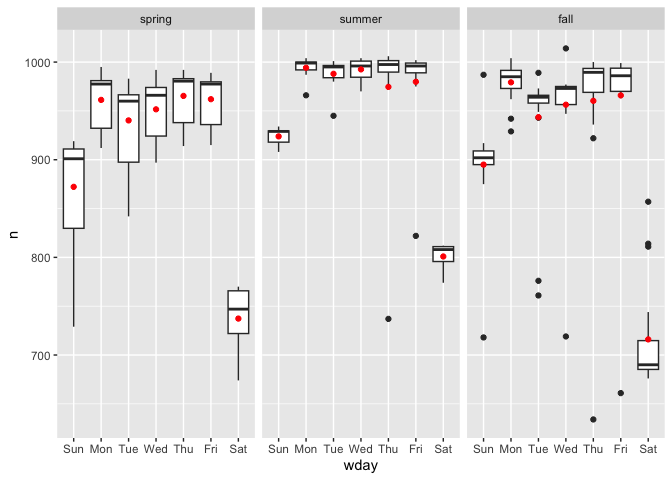
\includegraphics{Chapter-22-Model-basics_files/figure-latex/unnamed-chunk-27-1.pdf}

\hypertarget{interaction-continuous-and-categorical}{%
\subsubsection{Interaction (continuous and
categorical)}\label{interaction-continuous-and-categorical}}

Trong trường hợp sim 3 vừa có continuous and categorical

\begin{Shaded}
\begin{Highlighting}[]
\FunctionTok{ggplot}\NormalTok{(sim3, }\FunctionTok{aes}\NormalTok{(x1, y)) }\SpecialCharTok{+} 
  \FunctionTok{geom\_point}\NormalTok{(}\FunctionTok{aes}\NormalTok{(}\AttributeTok{colour =}\NormalTok{ x2))}
\end{Highlighting}
\end{Shaded}

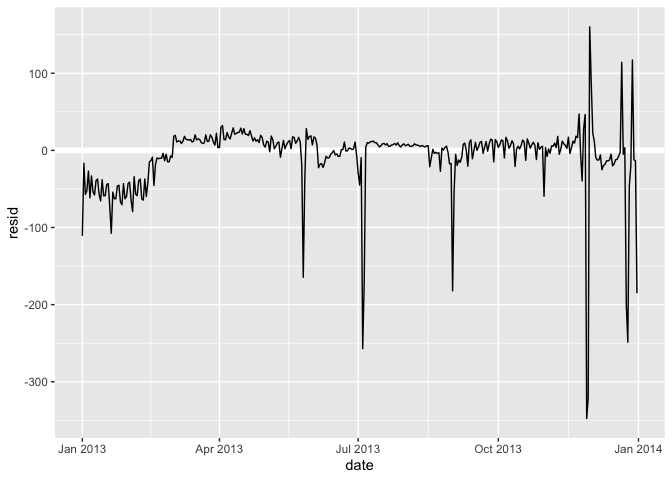
\includegraphics{Chapter-22-Model-basics_files/figure-latex/unnamed-chunk-28-1.pdf}

2 models có thể fit cho data này

\begin{Shaded}
\begin{Highlighting}[]
\NormalTok{mod1 }\OtherTok{\textless{}{-}} \FunctionTok{lm}\NormalTok{(y }\SpecialCharTok{\textasciitilde{}}\NormalTok{ x1 }\SpecialCharTok{+}\NormalTok{ x2, }\AttributeTok{data =}\NormalTok{ sim3)}
\NormalTok{mod2 }\OtherTok{\textless{}{-}} \FunctionTok{lm}\NormalTok{(y }\SpecialCharTok{\textasciitilde{}}\NormalTok{ x1 }\SpecialCharTok{*}\NormalTok{ x2, }\AttributeTok{data =}\NormalTok{ sim3)}
\end{Highlighting}
\end{Shaded}

(y \textasciitilde{} x1 + x2): y = a\_0 + a\_1*x1 + a\_2*x2

(y \textasciitilde{} x1 * x2): y = a\_0 + a\_1*x1 + a\_2*x2 +a\_12*x1*x2

Tạo bảng prediction

\begin{Shaded}
\begin{Highlighting}[]
\NormalTok{grid }\OtherTok{\textless{}{-}}\NormalTok{ sim3 }\SpecialCharTok{\%\textgreater{}\%} 
  \FunctionTok{data\_grid}\NormalTok{(x1, x2) }\SpecialCharTok{\%\textgreater{}\%} 
  \FunctionTok{gather\_predictions}\NormalTok{(mod1, mod2)}
\NormalTok{grid}
\end{Highlighting}
\end{Shaded}

\begin{verbatim}
## # A tibble: 80 x 4
##    model    x1 x2     pred
##    <chr> <int> <fct> <dbl>
##  1 mod1      1 a      1.67
##  2 mod1      1 b      4.56
##  3 mod1      1 c      6.48
##  4 mod1      1 d      4.03
##  5 mod1      2 a      1.48
##  6 mod1      2 b      4.37
##  7 mod1      2 c      6.28
##  8 mod1      2 d      3.84
##  9 mod1      3 a      1.28
## 10 mod1      3 b      4.17
## # ... with 70 more rows
\end{verbatim}

Graph

\begin{Shaded}
\begin{Highlighting}[]
\FunctionTok{ggplot}\NormalTok{(sim3, }\FunctionTok{aes}\NormalTok{(x1, y, }\AttributeTok{colour =}\NormalTok{ x2)) }\SpecialCharTok{+} 
  \FunctionTok{geom\_point}\NormalTok{() }\SpecialCharTok{+} 
  \FunctionTok{geom\_line}\NormalTok{(}\AttributeTok{data =}\NormalTok{ grid, }\FunctionTok{aes}\NormalTok{(}\AttributeTok{y =}\NormalTok{ pred)) }\SpecialCharTok{+} 
  \FunctionTok{facet\_wrap}\NormalTok{(}\SpecialCharTok{\textasciitilde{}}\NormalTok{ model)}
\end{Highlighting}
\end{Shaded}

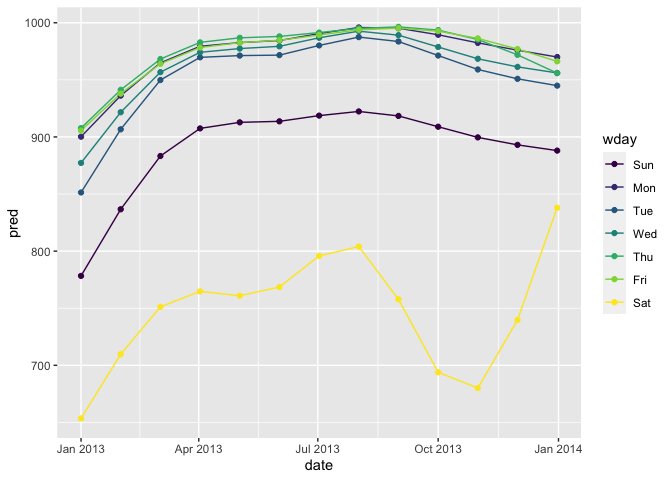
\includegraphics{Chapter-22-Model-basics_files/figure-latex/unnamed-chunk-31-1.pdf}

Xem residual của từng line

\begin{Shaded}
\begin{Highlighting}[]
\NormalTok{sim3 }\OtherTok{\textless{}{-}}\NormalTok{ sim3 }\SpecialCharTok{\%\textgreater{}\%} 
  \FunctionTok{gather\_residuals}\NormalTok{(mod1, mod2)}

\FunctionTok{ggplot}\NormalTok{(sim3, }\FunctionTok{aes}\NormalTok{(x1, resid, }\AttributeTok{colour =}\NormalTok{ x2)) }\SpecialCharTok{+} 
  \FunctionTok{geom\_point}\NormalTok{() }\SpecialCharTok{+} 
  \FunctionTok{facet\_grid}\NormalTok{(model }\SpecialCharTok{\textasciitilde{}}\NormalTok{ x2)}
\end{Highlighting}
\end{Shaded}

\includegraphics{Chapter-22-Model-basics_files/figure-latex/unnamed-chunk-32-1.pdf}

\hypertarget{interactions-2-continuous}{%
\subsubsection{Interactions (2
continuous)}\label{interactions-2-continuous}}

\begin{Shaded}
\begin{Highlighting}[]
\NormalTok{mod1 }\OtherTok{\textless{}{-}} \FunctionTok{lm}\NormalTok{(y }\SpecialCharTok{\textasciitilde{}}\NormalTok{ x1 }\SpecialCharTok{+}\NormalTok{ x2, }\AttributeTok{data =}\NormalTok{ sim4)}
\NormalTok{mod2 }\OtherTok{\textless{}{-}} \FunctionTok{lm}\NormalTok{(y }\SpecialCharTok{\textasciitilde{}}\NormalTok{ x1 }\SpecialCharTok{*}\NormalTok{ x2, }\AttributeTok{data =}\NormalTok{ sim4)}

\NormalTok{grid }\OtherTok{\textless{}{-}}\NormalTok{ sim4 }\SpecialCharTok{\%\textgreater{}\%} 
  \FunctionTok{data\_grid}\NormalTok{(}
    \AttributeTok{x1 =} \FunctionTok{seq\_range}\NormalTok{(x1, }\DecValTok{5}\NormalTok{), }
    \AttributeTok{x2 =} \FunctionTok{seq\_range}\NormalTok{(x2, }\DecValTok{5}\NormalTok{) }
\NormalTok{  ) }\SpecialCharTok{\%\textgreater{}\%} 
  \FunctionTok{gather\_predictions}\NormalTok{(mod1, mod2)}
\NormalTok{grid}
\end{Highlighting}
\end{Shaded}

\begin{verbatim}
## # A tibble: 50 x 4
##    model    x1    x2   pred
##    <chr> <dbl> <dbl>  <dbl>
##  1 mod1   -1    -1    0.996
##  2 mod1   -1    -0.5 -0.395
##  3 mod1   -1     0   -1.79 
##  4 mod1   -1     0.5 -3.18 
##  5 mod1   -1     1   -4.57 
##  6 mod1   -0.5  -1    1.91 
##  7 mod1   -0.5  -0.5  0.516
##  8 mod1   -0.5   0   -0.875
##  9 mod1   -0.5   0.5 -2.27 
## 10 mod1   -0.5   1   -3.66 
## # ... with 40 more rows
\end{verbatim}

vẽ

\begin{Shaded}
\begin{Highlighting}[]
\FunctionTok{ggplot}\NormalTok{(grid, }\FunctionTok{aes}\NormalTok{(x1, x2)) }\SpecialCharTok{+} 
  \FunctionTok{geom\_tile}\NormalTok{(}\FunctionTok{aes}\NormalTok{(}\AttributeTok{fill =}\NormalTok{ pred)) }\SpecialCharTok{+} 
  \FunctionTok{facet\_wrap}\NormalTok{(}\SpecialCharTok{\textasciitilde{}}\NormalTok{ model)}
\end{Highlighting}
\end{Shaded}

\includegraphics{Chapter-22-Model-basics_files/figure-latex/unnamed-chunk-34-1.pdf}

Không thấy rõ model nào fit tốt hơn

\begin{Shaded}
\begin{Highlighting}[]
\FunctionTok{ggplot}\NormalTok{(grid, }\FunctionTok{aes}\NormalTok{(x1, pred, }\AttributeTok{colour =}\NormalTok{ x2, }\AttributeTok{group =}\NormalTok{ x2)) }\SpecialCharTok{+} 
  \FunctionTok{geom\_line}\NormalTok{() }\SpecialCharTok{+}
  \FunctionTok{facet\_wrap}\NormalTok{(}\SpecialCharTok{\textasciitilde{}}\NormalTok{ model)}
\end{Highlighting}
\end{Shaded}

\includegraphics{Chapter-22-Model-basics_files/figure-latex/unnamed-chunk-35-1.pdf}

\begin{Shaded}
\begin{Highlighting}[]
\FunctionTok{ggplot}\NormalTok{(grid, }\FunctionTok{aes}\NormalTok{(x2, pred, }\AttributeTok{colour =}\NormalTok{ x1, }\AttributeTok{group =}\NormalTok{ x1)) }\SpecialCharTok{+} 
  \FunctionTok{geom\_line}\NormalTok{() }\SpecialCharTok{+}
  \FunctionTok{facet\_wrap}\NormalTok{(}\SpecialCharTok{\textasciitilde{}}\NormalTok{ model)}
\end{Highlighting}
\end{Shaded}

\includegraphics{Chapter-22-Model-basics_files/figure-latex/unnamed-chunk-35-2.pdf}

\end{document}
